% \documentclass{beamer}
% \usetheme{Szeged}

% \begin{document}

%-------------------------------------------------------------------------------
%							FITH SECTION
%-------------------------------------------------------------------------------


\section{Conclusion}
% Conclusion

\subsection{Sur l'apprentissage}
\begin{frame}
    \frametitle{Bilan de l'apprentissage}
    Par ordre croissant de reussite:
    \begin{enumerate}
        \item \textbf{Régression 1D} : Permet de détecter la hauteur du créneau %sur la densité d'un domaine 1D (avec la meilleure corrélation de tous les apprentissages). Elle n'a cependant pas été capable de détecter la position du créneau, probablement dû au caractère mal posé du problème inverse.
        \item \textbf{Classification 2D} : Permet de localiser l'ordonnée du créneau %en le situant par rapport aux sources sur la gauche d'un domaine 2D. En augmentant leur nombre et en plaçant certaines sources en haut (ou en bas) du domaine, on pourrait localiser avec plus de finesse l'abscisse et l'ordonnée du créneau.
        \item \textbf{Régression 2D} : Permet de prédire tous les attributs essentiels du créneau (abscisse, ordonnée, et hauteur)%, tout ceci avec une très forte précision (score personnalisé s'élevant à 93 \%). 
      \end{enumerate}
\end{frame}

\subsection{Generale}
\begin{frame}
    \frametitle{Bilan du stage}
    \begin{figure}
        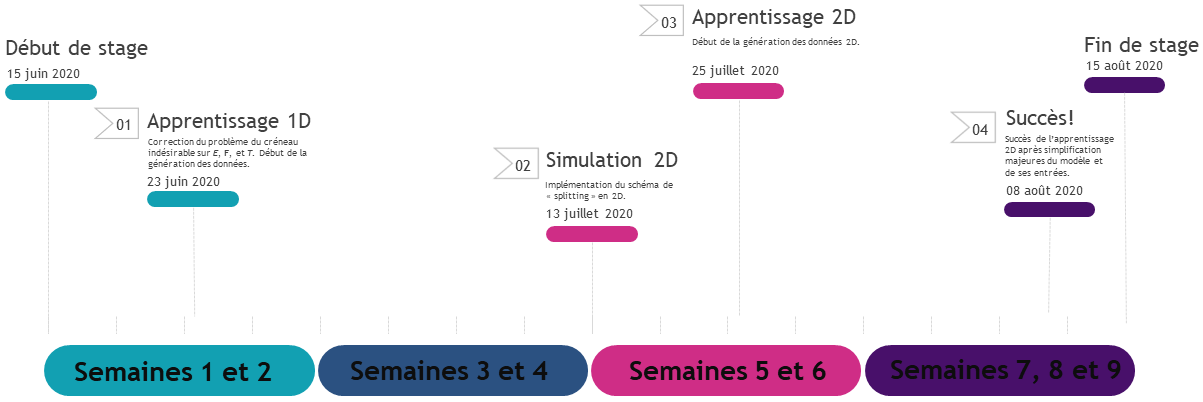
\includegraphics[width=10cm]{MilestonesRoadmap}       
        \caption{Points tournants du le stage}
    \end{figure}
\end{frame}

\begin{frame}
    \frametitle{Apports et enseignements}
    \begin{itemize}
        \item Developpement C++ et Python   % Mettre en pratique les connaissances de CSMI
        \item Equations aux derivees partielles % technique de verification
        \item Reseaux de neurones % (Keras, Tensorflow, learning rate)
        \item Experience dans un milieu de recherche % J'ai apprecieer travailler sur IA+EDP
        % \item Point negatif: Manque de coordination (A cause du COVID)
    \end{itemize}
\end{frame}


% \end{document}
